% Current file is main.tex

%------------------------------------------------------------------------%
% Vorlage für Praxisarbeiten (o. Ä.) an der DHBW
%
% Autoren: Finn Hülsbusch, Daniel Kerger
% Version: 1.0.0
% Datum:   11.05.2020
%------------------------------------------------------------------------%


% -- Präambel mit Angaben zum Dokument
% Current file is content/00_LaTeX/preamble.tex

%------------------------------------ Informationen ------------------------------------%
% Bei diesem Dokument handelt es sich um die Präambel des Dokuments. 
% Strukur der Präambel:
% 01: Allgemeines
% 02: Mathematik
% 03: Verzeichnisse
% 04: Quellenverwaltung
% 05: Bilder
% 06: Tabellen
% 07: Listen
% 08: Listings
% 09: Eigene Umgebungen
% 10: Abkürzungen 
% 11: Referenzen
% 12: Variablen
% 13: Sonstige 


%------------------------------------ Allgemeines ------------------------------------%
% 1.	Dokumentenklasse
% 2.	Sprache und Umlaute
% 3.	Zeilenabstand
% 4.	Zeilenumbrüche und Seitenränder
% 5.	Absätze
% 6.	Schriftart
% 7.	Überschriften
% 8.	Automatische Seitenumbrüche von LaTeX

% -- Deklarierung der Dokumentenklasse scrreprt
\documentclass[
	fontsize=12pt,			% Leitlinien von der Schriftgröße 12.
	paper=A4,				% Papiergröße wird auf A4 festgelegt
	twoside=false,			% Zweiseitiger Druck wird deaktiviert
	listof=totoc,           % Tabellen- und Abbildungsverzeichnis in das Inhaltsverzeichnis
	index=totoc,			% Stichwortverzeichnis wird in das Inhaltsverzeichnis aufgenommen
	bibliography=totoc,		% Literaturverzeichnis wird in das Inhaltsverzeichnis aufnehmen
	titlepage,              % Titlepage-Umgebung anstatt \maketitle
	headsepline,            % Horizontale Linie unter Kolumnentitel
	abstracton,             % Überschrift einschalten, Abstract muss in {abstract}-Umgebung stehen
	hidelinks,				% Boxen um klickbare Links werden entfernt
	ngerman,				% Sprache wird auf Deutsch festgelegt
	english					% Englisch als weiter Sprache hinzufügen
]{scrreprt}             	% Verwendung von KOMA-Report


% -- Einstellung der Sprache des Dokuments und die Darstellung von mathematischen Symbolen und Eingabemöglichkeit von Umlauten
\usepackage[
	main = ngerman,							% Sprache wird auf Deutsch festgelegt
	english									% Englisch wird unterstützt
]{babel}									
\usepackage[T1]{fontenc}					% Voraussetzung für LaTeX Fonts in westeuropäischer Codierung
\usepackage[utf8]{inputenc}					% UTF8 wird unterstützt
\usepackage[activate]{microtype}      		% Trennung von Wörtern wird besser umgesetzt
\usepackage{lmodern}         				% Nicht-gerasterte Schriftarten (bei MikTeX erforderlich)
\usepackage[babel]{csquotes}  				% Anführungszeichen + Zitate


% -- Einstellungen am Zeilenabstand
\usepackage[onehalfspacing]{setspace}		% Zeilenabstand \singlespacing, \onehalfspaceing, \doublespacing
\usepackage{scrlayer-scrpage} 	   			% Paket für die Gestaltung von Fuß- und Kopfzeilen


% -- Einstellungen für den Zeilenumbruch, Seitenränder und mehr
\usepackage[
	left=2.7cm, 							% Ränder links werden eingestellt
	right=2.5cm,							% Ränder rechts werden eingestellt
	top=2.5cm,  							% Ränder oben werden eingestellt
	bottom=2.5cm,							% Ränder unten werden eingestellt
	includeheadfoot							% Schließt den Kopf und den Fuß in den druckbaren Bereich mit ein
]{geometry}                 


% Layout für die Absätze
\setlength{\parindent} {0.0em}
\setlength{\parskip} {1.5ex plus0.5ex minus0.5ex}   	% Setzt den Abstand zwischen 2 Absätzen 


% -- Einstellung der Schriftart
\usepackage[scaled=.95]{helvet}
\renewcommand*\familydefault{\sfdefault} 				% Serifenlose Schrift 


% ---- Abstand verkleinern von der Überschrift 
\renewcommand*{\chapterheadstartvskip}{\vspace*{.5\baselineskip}}


% -- Automatische Seitenumbrüche von LaTeX verbessern
\widowpenalty10000
\clubpenalty10000


%------------------------------------ Mathematik ------------------------------------%
% 1.	Erweiterungen des Mathe-Satzes
% 2.	SI-Einheiten

% -- Einstellungen für Mathematik
\usepackage[sumlimits, intlimits]{amsmath}  % Bei Integralen und Summen werden die Zahlen oben drüber geschrieben 
\usepackage{amssymb}						% Erweiterung vom Mathe-Satz durch Symbole	
\usepackage{amsfonts}						% Zusätzliche Schriftarten für den Mathe-Satz, sowie neue Symbole
\usepackage{MnSymbol}   					% Für Symbole, die in amssymb nicht enthalten sind.						
\usepackage{mathtools}						% Verbesserung der Anzeige von mathematischen Symbolen
\usepackage{xfrac}							% Erweiterung der Brüche im Mathemodus
\usepackage{mathrsfs}						% Raph Smith’s Formal Script Schriftart i Mathe-Modus


% -- Einstellungen der SI Einheiten werden festgelegt.
\usepackage{siunitx}
\sisetup{
	locale=DE, 								% Sprache wird auf Deutsch festgelegt
	range-phrase={~bis~}, 
	output-decimal-marker={,}				% Damit ein Komma und kein Punkt verwendet wird.
} 


%------------------------------------ Verzeichnisse ------------------------------------%
% 1.	Inhaltsverzeichnis
% 2.	Stichwortverzeichnis
% 3.	Verbesserung der Übersetzung
% 4.	Anhang
% 5.	Glossar

% -- Einstellungen am Inaltsverzeichnis
\usepackage{titletoc}				  		% Paket für die Anpassungen am Inhaltsverzeichnis und dem Anhang
\contentsmargin{0.75cm}       		  		% Abstand im Inhaltsverzeichnis zw. Punkt und Seitenzahl


% -- Einstellungen für das Stichwortverzeichnis
\usepackage{makeidx}						% Paket für das Stichwortverzeichnis
\makeindex							


% -- Verbesserung der Übersetzung
\usepackage{bookmark}						% Nur ein LaTeX-Durchlauf für die Aktualisierung von Verzeichnissen nötig


% -- Einstellungen für den Anhang
\usepackage[titletoc]{appendix} %Fügt "Anhang" in TOC ein. 


% -- Einstellungen für das Glossar
\usepackage[
	nonumberlist,							% Keine Seitenzahlen im Glossar
	toc										% Aufnahme in das Inhaltsverzeichniss 
]{glossaries}

%------------------------------------ Quellenverwaltung ------------------------------------%
% 1.	Einstellungen von Biblatex
% 2.	Speicherort der Bibtex-Datei
% 3.	Umbruchgrenzen im Literaturverzeichnis

% -- Einstellungen für Biblatex
\usepackage[
	backend = biber,                		% Verweis auf biber
	language = auto,						% Sprache wird automatisch festgelegt
	style = numeric-comp,                	% Nummerierung der Quellen mit Zahlen
	bibencoding = utf8,						% UTF8 wird in biblatex aktiviert
	sorting = none,                 		% none = Sortierung nach der Erscheinung im Dokument
	sortcites = true,               		% Sortiert die Quellen innerhalb eines cite-Befehls
	block = space,                  		% Extra Leerzeichen zwischen Blocks
	hyperref = true,                		% Links sind klickbar auch in der Quelle
	giveninits = true,              		% Vornamen werden abgekürzt
	doi=true,                      			% DOI anzeigen
	isbn=true,                     			% ISBN anzeigen
	alldates=short                  		% Datum immer als DD.MM.YYYY anzeigen
]{biblatex}

% -- Einstellung des Dateipfades der Bibtex-Datei
\addbibresource{content/sources.bib}		% Speicherort der Quellendatei


% -- Einstellung der Umbruchgrenzen im Literaturverzeichnis
\setcounter{biburlnumpenalty}{3000}     	% Umbruchgrenze für Zahlen
\setcounter{biburlucpenalty}{6000}      	% Umbruchgrenze für Großbuchstaben
\setcounter{biburllcpenalty}{9000}     		% Umbruchgrenze für Kleinbuchstaben
\DeclareNameAlias{default}{family-given}	% Nachname vor dem Vornamen


% -- Änderungen am Layout der Quellen im Literaturverzeichnis 
\AtBeginBibliography{										% Schrägstrich zwischen den Autorennamen
	\renewcommand{\multinamedelim}{\addslash\space} 		
	\renewcommand{\finalnamedelim}{\multinamedelim}
}  

\DefineBibliographyStrings{german}{							% Ändern des Titels von "besucht am":
	urlseen = {Einsichtnahme:},                      
}


%------------------------------------ Bilder ------------------------------------%
% 1.	Grundlegende Pakete für Bilder
% 2.	Bildunterschriften
% 3. 	Allgemeine Verbesserungen

% -- Benötigte Pakete für Bilder
\usepackage{wrapfig}						% Wrapfigureumgebung wird ermöglicht
\usepackage{graphicx}						% Standardpaket für Bilder
\usepackage{caption}						% Bildunterschriften werde eingebunden


% -- Einstellungen für Bilder
\graphicspath{{images/}} 					% Standardpfad für Bilder wird angepasst, sodass nur noch der Dateiname des Bildes angegeben werden muss


% -- Einstellungen für Unterüberschriften 
\addtokomafont{caption}{\small} 			% Bildunterschriften werden etwas kleiner dargestellt
\usepackage[list=true]{subcaption} 			% Subbilder des Paketes subifigure werden im Abbildungsverzeichniss dargestellt 


\usepackage{float} 							% Verbesserung der floating-Option bei Bildern durch hinzufügen von "H" als Option


%------------------------------------ Tabellen ------------------------------------%
% 1.	Grundlegende Pakete für Tabellen
% 2.	Zeilen- und Linienabstände 

% -- Benötigte Pakete für Tabellen
\usepackage{booktabs}  						% Für schönere Tabellen. Enthält neue Befehle wie \midrule
\usepackage{multirow}  						% Mehrzeilige Tabellen
\usepackage{longtable}						% Verbesserte Tabellenumgebung
\usepackage{array}							% Erweitert die Tabellenumgebung
\usepackage{makecell}						% Ermöglichen von Umbrüchen in Tabellen

% -- Einstellungen für Tabellen
\setlength{\tabcolsep}{10pt}				% Abstand des Inhalts zur Linie
\renewcommand{\arraystretch}{1.25}			% Abstand der Zeilen wird erhöht 1.0 ist default


%------------------------------------ Aufzählungen ------------------------------------%
% 1.	Grundlegende Pakete für Aufzählungen

% -- Benötigte Pakete für Aufzählungen
\usepackage{enumitem}		% Ermöglicht Listen, wie itemize und enumerate


%------------------------------------ Listings ------------------------------------%
% 1.	Grundlegende Pakete für Listings
% 2.	Importierung des SourceCodeStyles
% 3.	Sonstige Einstellungen

% -- Grundlegende Pakete für Listings
\usepackage{scrhack}                    					% Hack zur Verw. von listings in KOMA-Script
\usepackage{listings}                 					  	% Darstellung von Quellcode
\usepackage{xcolor}                     					% Einfache Verwendung von Farben
\usepackage{algorithm}                  					% Für Algorithmen-Umgebung (ähnlich wie lstlistings Umgebung)
\usepackage{algpseudocode}              					% Für Pseudocode. Füge "[noend]" hinzu, wenn du kein "endif", etc. haben willst.


% -- Importierung des SourceCodeStyles
% Current file is content/00_LaTeX/sourceCodeStyle/sourceCodeStyle.tex

% -- Default Farben für den Quellcode
\definecolor{DefaultGruen}{rgb}{0.3,0.5,0.4}
\definecolor{DefaultBlau}{rgb}{0.0,0.0,1.0}

% -- Default Listing-Style
\lstset{
	% Das Paket "listings" kann kein UTF-8. Deswegen werden hier 
	% die häufigsten Zeichen definiert (ä,ö,ü,...)
	literate=%
		{á}{{\'a}}1 {é}{{\'e}}1 {í}{{\'i}}1 {ó}{{\'o}}1 {ú}{{\'u}}1
		{Á}{{\'A}}1 {É}{{\'E}}1 {Í}{{\'I}}1 {Ó}{{\'O}}1 {Ú}{{\'U}}1
		{à}{{\`a}}1 {è}{{\`e}}1 {ì}{{\`i}}1 {ò}{{\`o}}1 {ù}{{\`u}}1
		{À}{{\`A}}1 {È}{{\'E}}1 {Ì}{{\`I}}1 {Ò}{{\`O}}1 {Ù}{{\`U}}1
		{ä}{{\"a}}1 {ë}{{\"e}}1 {ï}{{\"i}}1 {ö}{{\"o}}1 {ü}{{\"u}}1
		{Ä}{{\"A}}1 {Ë}{{\"E}}1 {Ï}{{\"I}}1 {Ö}{{\"O}}1 {Ü}{{\"U}}1
		{â}{{\^a}}1 {ê}{{\^e}}1 {î}{{\^i}}1 {ô}{{\^o}}1 {û}{{\^u}}1
		{Â}{{\^A}}1 {Ê}{{\^E}}1 {Î}{{\^I}}1 {Ô}{{\^O}}1 {Û}{{\^U}}1
		{œ}{{\oe}}1 {Œ}{{\OE}}1 {æ}{{\ae}}1 {Æ}{{\AE}}1 {ß}{{\ss}}1
		{ű}{{\H{u}}}1 {Ű}{{\H{U}}}1 {ő}{{\H{o}}}1 {Ő}{{\H{O}}}1
		{ç}{{\c c}}1 {Ç}{{\c C}}1 {ø}{{\o}}1 {å}{{\r a}}1 {Å}{{\r A}}1
		{€}{{\euro}}1 {£}{{\pounds}}1 {«}{{\guillemotleft}}1
		{»}{{\guillemotright}}1 {ñ}{{\~n}}1 {Ñ}{{\~N}}1 {¿}{{?`}}1,
	breaklines=true,        				   % Breche lange Zeilen um 
	breakatwhitespace=true, 				   % Wenn möglich, bei Leerzeichen umbrechen
	% Symbole für Zeilenumbruch einfügen
	prebreak=\raisebox{0ex}[0ex][0ex]{\ensuremath{\rhookswarrow}},
	postbreak=\raisebox{0ex}[0ex][0ex]{\ensuremath{\rcurvearrowse\space}},
	tabsize=4,                                 % Setze die Breite eines Tabs
	basicstyle=\ttfamily\small,                % Grundsätzlicher Schriftstyle
	columns=fixed,                             % Besseres Schriftbild
	numbers=left,                              % Nummerierung der Zeilen
	%frame=single,                             % Umrandung des Codes
	showstringspaces=false,                    % Keine Leerzeichen hervorheben
	keywordstyle=\color{blue},
	ndkeywordstyle=\bfseries\color{darkgray},
	identifierstyle=\color{black},
	commentstyle=\itshape\color{DefaultGruen}, % Kommentare in eigener Farbe
	stringstyle=\color{DefaultBlau},           % Strings in eigener Farbe,
	captionpos=b                               % Bild*unter*schrift
}

% -- Laden der zusätzlichen Styles
% Current file is content/00_LaTeX/sourceCodeStyle/languages/C&C++.tex

% -- Eigene Farben für den Style
\definecolor{C++Lila}{HTML}{A640FF}
\definecolor{C++Orange}{HTML}{D69D85}
\definecolor{C++Blau}{HTML}{569CD6}
\definecolor{C++DunkelBlau}{HTML}{0E4583}
\definecolor{C++Mint}{HTML}{B8D7A3}
\definecolor{C++Creme}{HTML}{DCDCAA}
\definecolor{C++Gruen}{HTML}{57A64A}
\definecolor{C++Tuerkis}{HTML}{4EC9B0}

% -- Eigener C/++-Style für den Quellcode
\renewcommand{\ttdefault}{pcr}               % Schriftart, welche auch fett beinhaltet
\lstdefinestyle{EigenerC++Style}{
	language=C++,			% Standardsprache des Quellcodes
    columns=flexible,
	morekeywords={nullptr},
	% Enumerators (Mint)
	morekeywords=[2]{},
    % Methoden (Cremefarben)
	morekeywords=[3]{},
	% Extra Keywords (Lila)
	morekeywords=[4]{},
	% Noch mehr Keywords (Gruen)
	morekeywords=[5]{},
    keywordstyle=\bfseries\color{C++DunkelBlau},
    keywordstyle=[2]\color{C++Mint},
    keywordstyle=[3]\color{C++Creme},
    keywordstyle=[4]\color{C++Lila},
    keywordstyle=[5]\color{C++Tuerkis},
	commentstyle=\itshape\color{C++Gruen},
	stringstyle=\color{C++Orange}
}
% Current file is content/00_LaTeX/sourceCodeStyle/languages/Java.tex

% -- Eigene Farben für den Style
\definecolor{JavaLila}{rgb}{0.4,0.1,0.4}
\definecolor{JavaGruen}{rgb}{0.3,0.5,0.4}
\definecolor{JavaBlau}{rgb}{0.0,0.0,1.0}

% -- Eigener JAVA-Style für den Quellcode
\renewcommand{\ttdefault}{pcr}               % Schriftart, welche auch fett beinhaltet
\lstdefinestyle{EigenerJavaStyle}{
	language=Java,                             % Syntax Highlighting für Java
	%frame=single,                             % Umrandung des Codes
	keywordstyle=\bfseries\color{JavaLila},    % Keywords in eigener Farbe und fett
	commentstyle=\itshape\color{JavaGruen},    % Kommentare in eigener Farbe und italic
	stringstyle=\color{JavaBlau}               % Strings in eigener Farbe
}
% Current file is content/00_LaTeX/sourceCodeStyle/languages/JSON.tex

% -- Eigene Farben für den Style


% -- Eigener JSON-Style für den Quellcode

% Current file is content/00_LaTeX/sourceCodeStyle/languages/Python.tex

%-- Eigene Farben für den Style
\definecolor{PyKeywordsBlue}{HTML}{0000AC}
\definecolor{PyCommentGrey}{HTML}{808080}
\definecolor{PyStringGreen}{HTML}{008080}

% -- Eigener Python-Style für den Quellcode
\renewcommand{\ttdefault}{pcr}
\lstdefinestyle{EigenerPythonStyle}{
	language=Python,
	columns=flexible,
	keywordstyle=\bfseries\color{PyKeywordsBlue},
	commentstyle=\itshape\color{PyCommentGrey},
	stringstyle=\color{PyStringGreen}
}
% Current file is content/00_LaTeX/sourceCodeStyle/languages/XML&XSD.tex

% -- Eigene Farben für den Style
\definecolor{XMLGruen}{rgb}{0.3,0.5,0.4}

% -- Eigener XML/XSD-Style für den Quellcode
\renewcommand{\ttdefault}{pcr}
\lstdefinestyle{EigenerXSDStyle}{
	language=XML,                     
	stringstyle=\color{XMLGruen},
	morekeywords={
		encoding,
		xs:schema,
		xs:element,
		xs:complexType,
		xs:sequence,
		xs:attribute,
		xs:simpleContent,
		xs:extension base, 
		encoding,
		schema,
		element,
		complexType,
		sequence,
		attribute,
		simpleContent,
		extension base
	}
}  	% Weitere Details sind ausgelagert


% -- Sonstige Einstellungen für die Quellcodevorlage
\makeatletter                          						% Sorgt dafür, dass man @ in Namen verwenden kann.
															% Ansonsten gibt es in der nächsten Zeile einen Compilefehler.
\renewcommand{\ALG@name}{Algorithmus}   					% Umbenennen von "Algorithm" im Header der Listings.
\makeatother                            					% Zeichen wieder zurücksetzen
\renewcommand{\lstlistingname}{Listing} 					% Erlaubt das Umbenennen von "Listing" in anderen Titel.

\addto\extrasngerman{%
	\def\equationautorefname~#1\null{Gleichung~(#1)\null}
	\def\lstnumberautorefname{Zeile}
	\def\lstlistingautorefname{Listing}
	\def\algorithmautorefname{Algorithmus}
	% Damit einheitlich "Abschnitt 1.2[.3]" verwendet wird und nicht "Unterabschnitt 1.2.3"
	% \def\subsectionautorefname{Abschnitt}
}


%------------------------------------ Eigene Umgebungen ------------------------------------%
% 1.	Definitionsboxen

% -- Einstellungen für Definitionsboxen
\usepackage{amsthm}                     				% Liefert die Grundlagen für Theoreme
\usepackage[framemethod=tikz]{mdframed} 				% Boxen für die Umrandung
% Current file is content/00_LaTeX/miscellanious/highlightBoxes.tex

% -- Grundsätzliche Definition zum Style
\newtheoremstyle{defi}
  {\topsep}         % Abstand oben
  {\topsep}         % Abstand unten
  {\normalfont}     % Schrift des Bodys
  {0pt}             % Einschub der ersten Zeile
  {\bfseries}       % Darstellung von der Schrift in der Überschrift
  {:}               % Trennzeichen zwischen Überschrift und Body
  {.5em}            % Abstand nach dem Trennzeichen zum Body Text
  {\thmname{#3}}    % Name in eckigen Klammern
\theoremstyle{defi}

% -- Definition zum Strich vor einem Text
\newmdtheoremenv[
  hidealllines = true,       % Rahmen komplett ausblenden
  leftline = true,           % Linie links einschalten
  innertopmargin = 0pt,      % Abstand oben
  innerbottommargin = 4pt,   % Abstand unten
  innerrightmargin = 0pt,    % Abstand rechts
  linewidth = 3pt,           % Linienbreite
  linecolor = gray!40,       % Linienfarbe
]{defStrich}{Definition}     % Name des Formats "defStrich"

% -- Definition zum Eck-Kasten um einen Text
\newmdtheoremenv[
  hidealllines = true,                                                  % Rahmen komplett ausblenden
  innertopmargin = 6pt,                                                 % Abstand oben
  linecolor = gray!40,                                                  % Linienfarbe
  singleextra={                                                         % Eck-Markierungen für die Definition
    \draw[line width=3pt,gray!50,line cap=rect] (O|-P) -- +(1cm,0pt);
    \draw[line width=3pt,gray!50,line cap=rect] (O|-P) -- +(0pt,-1cm);
    \draw[line width=3pt,gray!50,line cap=rect] (O-|P) -- +(-1cm,0pt);
    \draw[line width=3pt,gray!50,line cap=rect] (O-|P) -- +(0pt,1cm);
  }
]{defEckKasten}{Definition}                                             % Name des Formats "defEckKasten"  	% Weitere Details sind ausgelagert


%------------------------------------ Abkürzungen ------------------------------------%
% 1.	Abkürzungen

% -- Einstellungen für Abkürzungen
\usepackage{acro}	%Abkürzungen werden nur gedruckt wenn sie gebraucht wurden
\acsetup{ 
	list/display = used, 				% zeigt nur genutzte Abkürzungen 
	list/sort = true, 					% sortiert alphabetisch 
}
% % Definition des neuen Befehls für das Einfügen der Abkürzung der Einheit


\DeclareAcroProperty{unit}

\NewAcroTemplate[list]{physics}{%
  \acronymsmapT{%
    \AcroAddRow{%
      \acrowrite{short}%
      &
      \acrowrite{unit}%
      &
      \acrowrite{list}%
      \tabularnewline
    }%
  }%
  \acroheading
  \acropreamble
  \par\noindent
  \setlength\LTleft{0pt}%
  \setlength\LTright{0pt}%
  \begin{longtable}{@{}lll@{\extracolsep{\fill}}l@{}}
    \AcronymTable
  \end{longtable}
}

\DeclareAcronym{f}{
  short = \ensuremath{f} ,
  long  = Frequenz ,
  unit  = \si{\hertz} ,
  tag   = physics
}
\DeclareAcronym{A}{
  short = \ensuremath{A} ,
  long  = Fläche ,
  unit  = \si{\metre^2} ,
  tag   = physics
}
\DeclareAcronym{C}{
  short = \ensuremath{C} ,
  long  = Kapazität ,
  unit  = \si{\farad} ,
  tag   = physics
}
\DeclareAcronym{F}{
  short = \ensuremath{F} ,
  long  = Kraft ,
  unit  = \si{\newton} ,
  tag   = physics
}

\NewAcroTemplate[list]{standard}{%
\acronymsmapT{%
  \AcroAddRow{%
	\acrowrite{short}%
	&
	\acrowrite{list}%
	\tabularnewline
  }%
}%
\acroheading
\acropreamble
\par\noindent
\setlength\LTleft{0pt}%
\setlength\LTright{0pt}%
\begin{longtable}{@{}lll@{\extracolsep{\fill}}l@{}}
  \AcronymTable
\end{longtable}
}


	
	\DeclareAcronym{CRISP-DM}{
  		short = CRISP-DM,
  		long  = Cross Industry Standard Process for Data Mining
	}
	
	\DeclareAcronym{ML}{
  		short = ML,
  		long  = Machine Learning
	}
	
	\DeclareAcronym{NYSE}{
  		short = NYSE,
  		long  = New York Stock Exchange
	}
	
	\DeclareAcronym{MACD}{
  		short = MACD,
  		long  = Moving Average Convergence Divergence
	}


%------------------------------------ Referenzen ------------------------------------%
% 1.	Varioref
% 2.	Hyperref
% 3.	Cleverev

% -- Varioref
\usepackage{varioref}


% -- Hyperref
\usepackage{hyperref}
\hypersetup{%
	linktocpage=true, 				% Nicht der Text sondern die Seitenzahlen in Verzeichnissen klickbar
	bookmarksnumbered=true 			% Überschriftsnummerierung im PDF Inhalt anzeigen.
}


% -- Cleverev
\usepackage[noabbrev]{cleveref}   	% Kein Erkennen von Abkürzungen 


%------------------------------------ Variablen ------------------------------------%
% 1.	Aufsetzten von Variablen

% -- Aufsetzen von Variablen
\usepackage{ifthen}
% Current file is content/00_LaTeX/variables/setupVariables

% -- Deklarierung von Variablen
% Hier werden Variablen, welche für zusätzliche Einstellungen im Dokument verwendet werden deklariert.
\newboolean{durchgehendeFussnoten}
\newboolean{sperrvermerkLangeVersion}
\newboolean{abgabeVersion}
\newboolean{englischeVersion}
\newboolean{anleitungDrucken}


%------------------------------------ Sonstiges ------------------------------------%
% 1.	Sonstige Pakete
% 2.	Sonstige Einstellungen

% Neue Überschrift für das Literaturverzeichnis auf Deutsch
\renewcaptionname{ngerman}{\bibname}{Literaturverzeichnis}
\newcaptionname{ngerman}{\lstlistlistingname}{Quellcodeverzeichnis}
\newcaptionname{english}{\lstlistlistingname}{List of Listings}

% -- Sonstige Pakete
\usepackage{lipsum}				% Paket für Blindtext
\usepackage{multicol}			% Mehrere Spalten auf einer Seite 
\usepackage{pdflscape}			% Rotieren einer einzelnen PDF-Seite in der landscape Umgebung
\usepackage{isodate}			% Datum wird in der Region entsprechend geändert

\pdfcompresslevel=0				% Geringer Komprimierung dadurch verbesserte Compiletime
\pdfobjcompresslevel=0			% Geringer Komprimierung dadurch verbesserte Compiletime 

% -- Änderungen an Schreibweisen und Silbentrennungen
% Current file is content/00_LaTeX/miscellanious/grammar.tex

% -- Hilfreiches
% Hier werden grundlegende Layoutfehler von LaTeX behoben:
% 1.    "z.B." mit kleinem Leeraum dazwischen (ohne wäre nicht korrekt)
% 2.    "d.h." mit kleinem Leeraum dazwischen (ohne wäre nicht korrekt)
\newcommand{\zB}{z.\,B. }
\newcommand{\dash}{d.\,h. }

% -- Silbentrennung 
% Hier werden Fehler der Silbentrennung behoben, oder Änderungen vorgenommen, falls die Standardwerte von LaTeX nicht gewünscht sind:
% 1.    "HANA" anstatt "HA-NA"
% 2.    "Graph-Script" anstatt "GraphS-cript"
 
\hyphenation{HANA}
\hyphenation{Graph-Script}

% -- Allgemeine Informationen zur Arbeit
\newcommand{\titel}{Vorhersage von Aktienkursen mithilfe von Machine Learning}
\newcommand{\titelheader}{Vorhersage von Aktienkursen durch ML}
\newcommand{\arbeit}{Praktische Data Science-Studie}

% -- Persönliche Angaben und DHBW
\newcommand{\vorname}{Johannes}
\newcommand{\nachname}{Knoll}
\newcommand{\matrikelnr}{8238685}
\newcommand{\kurs}{WWIMASE19A}
\newcommand{\studiengang}{Wirtschaftsinformatik(SE)}
\newcommand{\studienjahr}{2019}										% Datum in dem Format yyyy angeben
\newcommand{\abschluss}{Bachelor of Science}
\newcommand{\dhbwStandort}{Mannheim}					
\newcommand{\betreuerDhbw}{Prof. Dr. Tobias Günther}

% -- Angaben zum Zeitraum und der Abgabe
\newcommand{\abgabeOrt}{Mannheim}						
\newcommand{\abgabeDatum}{2022-04-11} 								% Datum in dem Format yyyy-mm-dd angeben
\newcommand{\bearbeitungszeitraumBeginn}{2022-03-22} 				% Datum in dem Format yyyy-mm-dd angeben
\newcommand{\bearbeitungszeitraumEnde}{2022-04-08} 					% Datum in dem Format yyyy-mm-dd angeben

% -- Angaben zu der Ausbildungsfirma
\newcommand{\firmaName}{SAP SE}
\newcommand{\firmaStrasse}{Dietmar-Hopp-Allee 16}
\newcommand{\firmaPlz}{69190 Walldorf, Deutschland}
\newcommand{\betreuerFirma}{B-Vorname B-Nachname}

% -- Zusätzliche Optionen 
\setboolean{durchgehendeFussnoten}{true}							% Die Fußnoten werden nicht nach jedem Kapitel neu gezählt
\setboolean{sperrvermerkLangeVersion}{true}							% Es soll eine lange Version des Sperrvermerks eingebunden werden
\setboolean{anleitungDrucken}{true} 								% Die Anleitung mit Beispielen wird gedruckt.
\setboolean{abgabeVersion}{false} 									% ToDo-Notes und andere Dokumente werden ausgeblendet. Dies ist die Abgabeversion.
\setboolean{englischeVersion}{false}								% Verwendung der englischen Version inklusive Satz. 
% Current file is content/00_LaTeX/variables/runVariables

\ifthenelse{\boolean{durchgehendeFussnoten}}
{
	\usepackage{chngcntr}
	\counterwithout{footnote}{chapter}
}
{}
\ifthenelse{\boolean{abgabeVersion}}
{
	% Pakete Für Todo Notes
	\usepackage[disable]{todonotes}
	\setlength {\marginparwidth }{2cm}      % Abstand für Todo Notizen
}
{
	% Pakete Für Todo Notes
	\usepackage{todonotes}
	\setlength {\marginparwidth }{2cm}      % Abstand für Todo Notizen
}

						% Einstellungen der Variablen werden ausgeführt

% -- Glossar
\makeglossaries														% Glossarfunktionen werden initialisiert
% Current file is content/07_appendix/glossary.tex

% Anleitung für das Glossar:
% 1. Normaler LaTeX Kompiliervorgang und nicht die Auxiliary Files löschen
% 2. In der Konsole den Befehl makeglossaries main ausführen
% 3. Abschließender LaTex Kompiliervorgang

% Glossareintraege --> referenz, name, beschreibung
% Aufruf mit \gls{...}
 
\newglossaryentry{Glossareintrag}
{   
    name={Glossareintrag},
    plural={Glossareinträge},
    description={Ein Glossar beschreibt verschiedenste Dinge in kurzen Worten}
}								% Glossareinträge werden ausgelesen

% -- Kopf- und Fußzeilen
% Current file is content/00_LaTeX/miscellanious/headerAndFooter.tex

% -- Metainformation für das PDF Dokument
% Hier werden die Metainformationen für das generierte PDF Dokument hinterlegt. Eingesehen werden können diese Informationen in Acrobat unter Datei -> Eigenschaften.
\hypersetup{
    pdftitle    = {\titel},
    pdfsubject  = {\arbeit},
    pdfauthor   = {\nachname, \vorname},
    pdfcreator  = {LaTeX}
}

% -- Definition der Kopf- und Fußzeilen
\clearscrheadfoot                               % Löschen von LaTeX Standard
\automark[section]{chapter}                     % Füllen von section und chapter
\renewcommand*{\chaptermarkformat}{}            % Entfernt die Kapitelnummer
\renewcommand*{\sectionmarkformat}{}            % Entfernt die Sectionnummer
% Angaben [für "plain"]{für "scrheadings"}
\ihead[]{\titelheader}                          % Kopfzeile links
\chead[]{}                                      % Kopfzeile mitte
\ohead[]{\rightmark}                            % Kopfzeile rechts
\ifoot[]{}                                      % Fußzeile links
\cfoot*{\sffamily\pagemark}                     % Fußzeile mitte
\ofoot[]{}                                      % Fußzeile rechts
\KOMAoptions{
   headsepline = 0.2pt,                         % Liniendicke Kopfzeile
   footsepline = false                          % Liniendicke Fußzeile
}				% Layout der Kopf- und Fußzeilen werden eingelesen

\begin{document}
	
	\ifthenelse{\boolean{englischeVersion}}
	{
		\selectlanguage{english}
	}
	{}

	\setlength{\parindent}{0pt}              						% Keine Paragraphen Einrückung.
	\setcounter{secnumdepth}{2}             						% Nummerierungstiefe fürs Inhaltsverzeichnis
	\setcounter{tocdepth}{1}             	    					% Tiefe des Inhaltsverzeichnisses. Ggf. so anpassen, dass das Verzeichnis auf eine Seite passt.
	\sffamily                                						% Serifenlose Schrift verwenden.
	
	% -- Einbinden des Deckblatts
	\singlespacing													% Einfacher Zeilenabstand
    % Current file is content/01_titlepage/tilepage.tex

\thispagestyle{empty}
\ifthenelse{\boolean{englischeVersion}}
{
	\begin{titlepage}
		\enlargethispage{4cm}
		\begin{figure}
			% \vspace*{-5mm} 
			\begin{minipage}{0.49\textwidth}
				\flushleft
				%\missingfigure[figheight=2.5cm, figcolor=white]{Insert company %logo here} 
				
\includegraphics[height=2.5cm]{images/logos/Logo_SAP.pdf} 
			\end{minipage}
			\hfill
			\begin{minipage}{0.49\textwidth}
				\flushright
				
\includegraphics[height=2.5cm]{images/logos/dhbw.pdf} 
			\end{minipage}
		\end{figure} 
		\vspace*{0.1cm}
		\begin{center}
			\huge{\textbf{\titel}}\\[1.5cm]
			\Large{\textbf{\arbeit}}\\[0.5cm]
			\normalsize{as part of the examination for the\\[1ex] \textbf{\abschluss}}\\[0.5cm]
			\Large{in \studiengang}\\[1ex]
			\normalsize{at the Baden-Wuerttemberg Cooperative State University \dhbwStandort}\\[1cm]
			\normalsize{by}\\[1ex] \Large{\textbf{\vorname\,\nachname}} \\[1cm]
			\normalsize{{\printdayoff\today}}\\[2.25cm]
			\begin{spacing}{0.8}
				\begin{tabular}{ll}
					\textbf{Date of submission}				\hspace{4.5cm}					& \printdate{\abgabeDatum}\\[0.2cm]
					\textbf{Handling period}       				&  \daterange{\bearbeitungszeitraumBeginn}{\bearbeitungszeitraumEnde}\\[0.2cm]
					\textbf{Matriculation number, Course}	   	&  \matrikelnr, \kurs\\[0.2cm]
					\textbf{Training company}              					 &  \firmaName\\
																							& \firmaStrasse \\
																							& \firmaPlz\\[0.2cm]
					\textbf{Supervisor of the training company}          &  \betreuerFirma\\[0.2cm]
					\textbf{Evaluator of the  Cooperative State University}    &  \betreuerDhbw\\[0.2cm]
				\end{tabular} 
			\end{spacing}
		\end{center}
	\end{titlepage}
}
{
\begin{titlepage}
	\enlargethispage{4cm}
	\begin{figure}
		% \vspace*{-5mm} 
		\begin{minipage}{0.49\textwidth}
			\flushleft
			%\missingfigure[figheight=2.5cm, figcolor=white]{Insert company %logo here} 
			
\includegraphics[height=2.5cm]{images/logos/Logo_SAP.pdf} 
		\end{minipage}
		\hfill
		\begin{minipage}{0.49\textwidth}
			\flushright
			
\includegraphics[height=2.5cm]{images/logos/dhbw.pdf} 
		\end{minipage}
	\end{figure} 
	\vspace*{0.1cm}
	\begin{center}
		\huge{\textbf{\titel}}\\[1.5cm]
		\Large{\textbf{\arbeit}}\\[0.5cm]
		\normalsize{im Rahmen der Prüfung zum\\[1ex] \textbf{\abschluss}}\\[0.5cm]
		\Large{des Studienganges \studiengang}\\[1ex]
		\normalsize{an der Dualen Hochschule Baden-Württemberg \dhbwStandort}\\[1cm]
		\normalsize{von}\\[1ex] \Large{\textbf{\vorname\,\nachname}} \\[1cm]
		\normalsize{{\printdayoff\today}}\\[2.25cm]
		\begin{spacing}{0.8}
			\begin{tabular}{ll}
				\textbf{Abgabedatum}				\hspace{4.5cm}					& \printdate{\abgabeDatum}\\[0.2cm]
				\textbf{Bearbeitungszeitraum}       				&  \daterange{\bearbeitungszeitraumBeginn}{\bearbeitungszeitraumEnde}\\[0.2cm]
				\textbf{Matrikelnummer, Kurs} 					   	&  \matrikelnr, \kurs\\[0.2cm]
				\textbf{Ausbildungsfirma}              					 &  \firmaName\\
																						& \firmaStrasse \\
																						& \firmaPlz\\[0.2cm]
				\textbf{Betreuer der Ausbildungsfirma}          &  \betreuerFirma\\[0.2cm]
				\textbf{Gutachter der Dualen Hochschule}    &  \betreuerDhbw\\[0.2cm]
			\end{tabular} 
		\end{spacing}
	\end{center}
\end{titlepage}
}						% Titelseite wird eingebunden
    \newcounter{savepage}											% Zähler für die römischen Zahlen wird erstellt.
    \pagenumbering{Roman} 											% Seitenzahlen werden durch römische Buchstaben gekennzeichnet
    \onehalfspacing													% Eineinhalbfacher Zeilenabstand
    
    % -- Einbinden der Erklärung
    % Current file is content/02_declaration/declaration.tex

\ifthenelse{\boolean{englischeVersion}}
{
	\chapter*{Declaration}
	Hereby I solemnly declare that this {\arbeit}, titled:
	\begin{quote}
		\textit{\titel}
	\end{quote}
	is entirely the product of my own scholarly work and I have indicated the thoughts adopted directly or indirectly from other sources at the appropriate places within the document. In addition I assure, that the printed version is equivalent to the submitted electronic one.
	\vspace{1cm}

	\abgabeOrt, the \printdate{\abgabeDatum} \\[0.5cm]
	{\makebox[6cm]{\hrulefill}}\\ 
	\nachname , \vorname
}
{
	\chapter*{Erklärung}
		Ich versichere hiermit, dass ich meine \arbeit{} mit dem Thema:
		\begin{quote}
			\textit{\titel}
		\end{quote}
		selbstständig verfasst und keine anderen als die angegebenen Quellen und Hilfsmittel benutzt habe. Ich versichere zudem, dass die eingereichte elektronische Fassung mit der gedruckten Fassung übereinstimmt. 
		\vspace{1cm}
		
		\abgabeOrt, den \printdate{\abgabeDatum} \\[0.5cm]
		{\makebox[6cm]{\hrulefill}}\\ 
		\nachname , \vorname
}

    
    % -- Einbinden des Sperrvermerks
    % % Current file is content/03_confidentiallyStatement/confidentiallyStatement.tex


\ifthenelse{\boolean{englischeVersion}}
{
	\chapter*{Confidentially Statement}
	The {\arbeit} on hand:
	\begin{quote}
		\textit{\titel}
	\end{quote}
 	contains internal resp.\ confidential data of {\firmaName}. It is intended solely for inspection by the assigned examiner, the head of the {\studiengang} department and, if necessary, the Audit Committee of the Baden-Wuerttemberg Cooperative State University \abgabeOrt. It is strictly forbidden
  	\begin{itemize}
		\item to distribute the content of this paper (including data, figures, tables, charts etc.) as a whole or in extracts,
		\item to make copies or transcripts of this paper or of parts of it,
		\item to display this paper or make it available in digital, electronic or virtual form.
  	\end{itemize}
	Exceptional cases may be considered through permission granted in written form by the author and {\firmaName}.
}
{
	\chapter*{Sperrvermerk}
	\ifthenelse{\boolean{sperrvermerkLangeVersion}}
	{
		Die vorliegende {\arbeit} mit dem Titel: 
		\begin{quote}
			\textit{\titel}
		\end{quote}
		enthält unternehmensinterne bzw. vertrauliche Informationen der {\firmaName}, ist deshalb mit einem Sperrvermerk versehen und wird ausschließlich zu Prüfungszwecken am Studiengang {\studiengang} der Dualen Hochschule Baden-Württemberg {\abgabeOrt} vorgelegt. Sie ist ausschließlich zur Einsicht durch den zugeteilten Gutachter, die Leitung des Studiengangs und ggf. den Prüfungsausschuss des Studiengangs bestimmt.  Es ist untersagt,
		\begin{itemize}
			\item den Inhalt dieser Arbeit (einschließlich Daten, Abbildungen, Tabellen, Zeichnungen usw.) als Ganzes oder auszugsweise weiterzugeben,
			\item Kopien oder Abschriften dieser Arbeit (einschließlich Daten, Abbildungen, Tabellen, Zeichnungen usw.) als Ganzes oder in Auszügen anzufertigen,
			\item diese Arbeit zu veröffentlichen bzw. digital, elektronisch oder virtuell zur Verfügung zu stellen. 
		\end{itemize}
		Jede anderweitige Einsichtnahme und Veröffentlichung – auch von Teilen der Arbeit – bedarf der vorherigen Zustimmung durch den Verfasser und {\firmaName}.
	}
	{
		Der Inhalt dieser Arbeit darf weder als Ganzes noch in Auszügen Personen außerhalb des Prüfungsprozesses und des Evaluationsverfahrens zugänglich gemacht werden, sofern keine anderslautende Genehmigung der Ausbildungsstätte vorliegt.
	}
}
    
    % -- Einbinden des Abstracts
    % % Current file is content/04_abstract/abstract-de.tex

\renewcommand{\abstractname}{Abstract} % Veränderter Name für das Abstract
\begin{abstract}
\begin{addmargin}[1.5cm]{1.5cm}        % Erhöhte Ränder, für Abstract Look
\thispagestyle{plain}                  % Seitenzahl auf der Abstract Seite

\begin{center}
\small\textit{- Deutsch -}             % Angabe der Sprache für das Abstract
\end{center}

\vspace{0.25cm}

Dies ist der Beginn des Abstracts. Für die finale Bachelorarbeit musst du ein Abstract in deinem Dokument mit einbauen. So, schreibe es am besten jetzt in Deutsch und Englisch. Das Abstract ist eine kurze Zusammenfassung mit ca. 200 bis 250 Wörtern.

\vspace{0.25cm}

Versuche in das Abstract folgende Punkte aufzunehmen: Fragestellung der Arbeit, methodische Vorgehensweise oder die Hauptergebnisse deiner Arbeit.


\end{addmargin}
\end{abstract}
    % % Current file is content/04_abstract/abstract-en.tex

\renewcommand{\abstractname}{Abstract} % Veränderter Name für das Abstract
\begin{abstract}
\begin{addmargin}[1.5cm]{1.5cm}        % Erhöhte Ränder, für Abstract Look
\thispagestyle{plain}                  % Seitenzahl auf der Abstract Seite

\begin{center}
\small\textit{- English -}             % Angabe der Sprache für das Abstract
\end{center}

\vspace{0.25cm}

This is the starting point of the Abstract. For the final bachelor thesis, there must be an abstract included in your document. So, start now writing it in German and English. The abstract is a short summary with around 200 to 250 words.

\vspace{0.25cm}

Try to include in this abstract the main question of your work, the methods you used or the main results of your work.


\end{addmargin}
\end{abstract}
    
    % -- Inhaltsverzeichnis
    \singlespacing													% Einfacher Zeilenabstand
    \tableofcontents												% Inhaltsverzeichnis wird erstellt

	% -- Verzeichnisse
	\renewcommand*{\chapterpagestyle}{plain}						% Kapitel-Style wird auf plain gestellt 
	\pagestyle{plain}												% Seiten-Style wird auf plain gestellt
	\ifthenelse{\boolean{englischeVersion}}{						% Einbindung des Formel- und Abkürzungsverzeichnisses mit angepassten Titeln
		\printacronyms[
			template=physics, 
			include=physics,
			name=List of Formulas
		]	
		\printacronyms[
			template=standard,
			exclude=physics, 
			name=List of Abbreviations
		]	
	}
	{
		\printacronyms[
			template=physics, 
			include=physics, 
			name=Formelverzeichnis
		]
		\printacronyms[
			template=standard, 
			exclude=physics, 
			name=Abkürzungsverzeichnis
		]
	}

	\listoffigures                         							% Erzeugen des Abbildungsverzeichnisses 
	\listoftables                          							% Erzeugen des Tabellenverzeichnisses
    % \lstlistoflistings                     							% Erzeugen des Listenverzeichnisses
    \setcounter{savepage}{\value{page}}								% Römische Seitenzahl wird für später gespeichert

	% -- Liste der zu erledigenden Punkte. Wichtig: Diese Liste muss vor der endgültigen Abgabe auskommentiert werden!
	% \listoftodos
    
    % -- Einbinden von den verschiedenen Kapiteln
    \cleardoublepage												% Beendet eine Seite
    \pagenumbering{arabic}                							% Arabische Seitenzahlen für den Hauptteil
    \setlength{\parskip}{0.5\baselineskip}  						% Abstand zwischen Absätzen wird geändert
    \rmfamily														% Schriftfamilie wird festgelegt
    \renewcommand*{\chapterpagestyle}{scrheadings}					% Kapitel-Style wird auf scrheadings gestellt 
    \pagestyle{scrheadings}											% Seiten-Style wird auf scrheadings gestellt
    \onehalfspacing													% Eineinhalbfacher Zeilenabstand
	\sffamily                               					 	% Serifenlose Schrift verwenden. 
	   
							% Beispielkapitel werden eingebunden
		\include{content/00_LaTeX/exampleProject/01_Einleitung}
		% \chapter{CRISP-DM}\label{chp:crisp}

Für den Verlauf dieser Arbeit wird eine Vorgehensweise aus dem Bereich des Data Mining verwendet, da diese gute Anwendungsmöglichkeiten für Projekte im Bereich ML bietet. Diese wird \ac{CRISP-DM} genannt. Der CRISP-DM wird verwendet, um den Lebenszyklus von Daten innerhalb eines Data Mining Projekts zu modellieren und ein dafür geeignetes Data Mining-Modell zu entwickeln. Der Prozess wird dabei in sechs verschiedene Phasen unterteilt, die unterschiedliche Ziele verfolgen \parencite[vgl.][S. 1]{.Wirth}.

\begin{figure}[H]
	\centering
	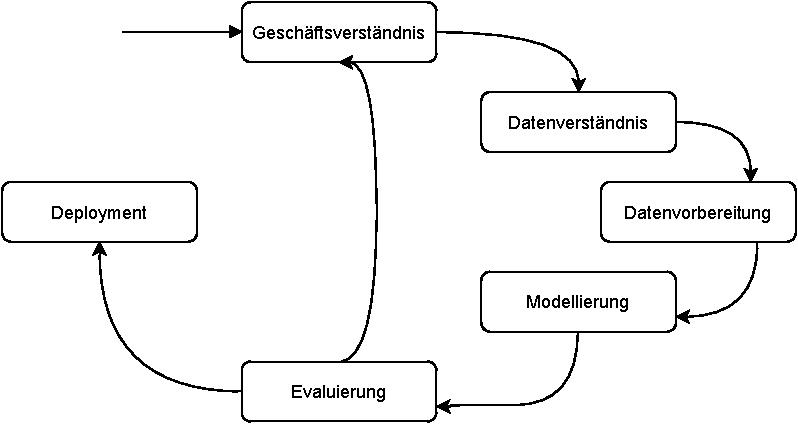
\includegraphics[scale=0.9]{images/CRISP.pdf}
	\caption{Ablauf eines CRISP-DM: Eigene Abbildung in Anlehnung an \parencite[][S. 5]{.Wirth}}
	\label{figure:ablauf-crisp-dm}
\end{figure}

In der ersten Phase geht es darum, die Ziele und die Anforderungen des Projekts zu untersuchen und diese in ein Data Mining-Problem zu übertragen. Anschließend muss sich der Entwickler mit den Daten vertraut machen. Dazu gehört beispielsweise das Gewährleisten der Datenqualität oder Erkenntnisse über die Daten, wie zum Beispiel deren Ursprung, zu sammeln. Nachdem die Daten untersucht wurden, werden diese so vorbereitet, dass sie in das ML-Modell eingefügt und mit ihnen gearbeitet werden kann. Dazu gehört unter anderem, doppelt vorkommende Datensätze oder Ausreißer zu entfernen. Anschließend kann damit begonnen werden, das Modell zu erstellen und die Ergebnisse zu evaluieren. Stellt sich nach der Evaluation heraus, dass nicht alle Anforderungen an das Modell erfüllt wurden, wird erneut damit begonnen, die Anforderungen zu definieren und die Daten zu analysieren, vorzubereiten und ein neues Modell zu erstellen. Erst nachdem alle Anforderungen erfüllt wurden, kann das Modell für den produktiven Gebrauch verwendet werden \parencite[vgl.][S. 5ff.]{.Wirth}.

% An diesen Phasen wird sich der Aufbau dieser Arbeit orientieren. In \vref{chp:problemanalyse-und-datenvorbereitung} wird damit begonnen, das vorliegende Problem zu analysieren und die Daten vorzubereiten. Anschließend werden in \vref{chp:entwicklung-verschiedener-loesungsansaetze} mögliche Modelle und Lösungsansätze entwickelt und in \vref{chp:evaluierung-2} analysiert und evaluiert. Da der Fokus dieser Arbeit auf der Erörterung der Sinnhaftigkeit von Anwendungen von Filtertechniken liegt, wird die Phase des Deployments nicht beachtet und ausgelassen. Auch eine erneute Analyse des Datenverständnisses wird in dieser Arbeit nicht thematisiert. Die Modellierung entspricht dabei der Entwicklung verschiedener Filtertechniken.
		\chapter{Geschäftsverständnis}\label{chp:geschaeftsverstaendnis}
Die Vorhersage von Aktienkursen ist ein wichtiges Finanzthema, das seit vielen Jahren die Aufmerksamkeit der Forscher auf sich zieht. Dabei wird davon ausgegangen, dass die in der Vergangenheit öffentlich zugänglichen grundlegenden Informationen einen gewissen prädiktiven Einfluss auf die zukünftigen Aktienrenditen haben \parencite[vgl.][S. 1]{.2013}.

Um die Aktienkurse vorherzusagen, existieren grundsätzlich zwei Methoden: die fundamentale und die technische Analyse \parencite[vgl.][S. 26f]{Petrusheva.2016}. Im Bereich der Fundamentalanalyse werden Handelsregeln auf Grundlage der Informationen über Makroökonomie und der Industrie des Unternehmens hergeleitet \parencite[vgl.][S. 1]{.2013}. Diese Art von Analyse geht davon aus, dass der Preis einer Aktie von ihrem inneren Wert und der erwarteten Kapitalrendite abhängt \parencite[vgl.][S. 453]{Tsang.2007}. Somit kann bei dieser Methode beispielsweise anhand der finanziellen Lage, der Liquidität oder der Attraktivität der Branche bewerten, ob eine Aktie Potenzial hat, in der kommenden Zeit zu steigen.

Bei der technischen Analyse hingegen werden Handelsregeln auf Grundlage historischer Daten von Aktienkursen und -volumen entwickelt \parencite[vgl.][S. 1]{.2013}. Diese Methode der Analyse bezieht sich auf verschiedene Methoden, die darauf abzielen, künftige Kursbewegungen anhand von vergangener Aktienkurse und -volumen vorherzusagen. Sie beruht auf der Annahme, dass sich in der Vergangenheit liegende Muster von Aktienkursen wiederholen und dass zukünftige Marktrichtungen anhand von der Untersuchung historischer Kursdaten ermittelt werden können \parencite[vgl.][S. 454]{Tsang.2007}. Bei dieser Methode werden Verfahren wie Trendanalysen, Chartmuster oder technische Indikatoren wie der \ac{MACD} oder Oszillatoren verwendet \parencite[vgl.][S. 293ff]{Mondello.2017}.

Mithilfe dieser Methoden werden Aktienkurse vorausgesagt, um beispielsweise den perfekten Zeitpunkt zu finden, um in die Investition eines Unternehmen einzusteigen oder eine Aktie zu verkaufen, um den Verlust von sinkenden Aktienkursen vorzubeugen. Da diese methodischen Analysen keine Garantie für den Verlauf einer Aktie garantieren, ergibt sich die Überlegung, Aktienkurse mithilfe eines ML-Modells vorherzusagen.
		\chapter{Datenverständnis}\label{chp:datenverstaendnis}
Bei dem verwendeten Datensatz handelt es sich um eine Sammlung von Unternehmen der \ac{NYSE}, von denen mehrere Kennzahlen des Aktienkurses und des Handelsvolumen gesammelt wurden. Innerhalb dieses Datensatzes wurden Informationen im Zeitraum vom 4. Januar 2010 bis zum 30. Dezember 2016 gesammelt. Dabei wurden nur die Wochentage Montag bis Freitag berücksichtigt, welche keine Feiertage waren. Folglich werden nur reguläre Handelstage an der Börse mit in die Berechnungen aufgenommen. Insgesamt wurden Daten von 501 Unternehmen gesammelt. Bei diesen Daten handelt es sich um folgende Variablen:

\begin{itemize}
    \item Das \textbf{Datum} verweist auf den Tag, an dem die Daten für ein bestimmtes Unternehmen gemessen wurden.
    \item In dem Feld \textbf{Symbol} ist die Abkürzung des Unternehmens gespeichert. Beispielsweise wird für das Unternehmen Amazon die Abkürzung ``AMZN'' hinterlegt.
    \item Der \textbf{Eröffnungskurs} gibt an, mit welchem Kurs die Aktien in den Handelstag gestartet ist.
    \item In der Variable \textbf{Schlusskurs} wird gespeichert, mit welchem Kurs die Aktie den Handelstag beendet hat.
    \item Das \textbf{Hoch} und \textbf{Tief} einer Aktien beschreiben den höchsten, beziehungsweise niedrigsten Kurs, den die Aktien an dem entsprechenden Tag verzeichnet hat.
    \item Das \textbf{Volumen} verweist auf die Anzahl der Aktien eines Unternehmens, die an dem Handelstag gehandelt wurden.
\end{itemize}

Da sich der Zeitraum der gesammelten Daten nur auf 2010 bis 2016 erstreckt, können mit diesem Modell nur Aktienkurse vorhergesagt werden, welche sich auch in diesem Zeitintervall befinden. Um den aktuellen Aktienkurs einer Aktie durch das Modell vorherzusagen, müssten auch aktuelle Daten gesammelt werden. Jedoch werden in \cref{chp:evaluierung} die tatsächlichen Schlusskurse im selbigen Zeitraum mit den von dem Modell vorhergesagten Schlusskursen verglichen.
		\chapter{Datenvorbereitung}\label{chp:datenvorbereitung}
Damit das ML-Modell erfolgreich trainiert werden kann, muss der verwendete Datensatz angepasst und gegebenenfalls bereinigt werden. Da innerhalb des verwendeten Datensatzes keine Duplikate oder fehlerhaften Daten enthalten sind, kann direkt damit begonnen werden, die Daten für das Trainieren des Modells vorzubereiten.

Der Datensatz wurde in einem Dataframe mithilfe der Programmiersprache Python gespeichert. Ein Dataframe ist eine zweidimensionale Datenstruktur, welches Daten in Tabellenform anordnet. Der Datensatz wurde zu Beginn direkt in ein Dataframe überführt. Anschließend wurden für die Berechnungen nicht benötigten Spalten der Datenstruktur entfernt. Dazu zählen beispielsweise das Symbol einer Aktie oder das Datum, welches auf den Handelstag hindeutet. Bei dem trainierten Modell werden jeweils nur die Schlusskurse einer bestimmten Aktie vorhergesagt. Dafür wird der Dataframe zu Beginn auf die Datensätze begrenzt, die dasselbe Symbol besitzen. Um beispielsweise den Aktienkurs von Amazon vorherzusagen, wird das ML-Modell auch nur mit historischen Daten von Amazon trainiert.

Im Anschluss wird der angepasste Datensatz mithilfe der Methode \textit{preprocessing.scale}\footnote{https://scikit-learn.org/stable/modules/generated/sklearn.preprocessing.scale.html} der Bibliothek sckit-learn\footnote{https://scikit-learn.org/stable/index.html} für das Trainieren des Modells standardisiert. Diese Standardisierung wird vorgenommen, damit die Rohdaten, die aus dem Datensatz stammen, so umgewandelt werden, damit sie in dem ML-Modell verarbeitet werden können. Dieser Prozess stellt einen Schritt dar, der in nahezu jedem ML-Projekt vollzogen werden muss.

Danach wird der standardisierte Datensatz in einen großen und einen kleinen Teil aufgeteilt. Der kleine Teil wird im weiteren Verlauf des Projekts verwendet, um einen Aktienkurs vorherzusagen. Die Größe des kleineren Teils beträgt dabei etwa 1\%, also etwa 18, der Gesamtgröße des Datensatzes. Auf dem großen Teil des Datensatzes wird ein Train-Test-Split mit der Methode \textit{train\_test\_split}\footnote{https://scikit-learn.org/stable/modules/generated/sklearn.model\_selection.train\_test\_split.html} durchgeführt. Diese Methode zerteilt den großen Datensatz in ein Trainings- und ein Test-Set. Mit dem Trainings-Set wird das ML-Modell trainiert. Das Test-Set hingegen wird verwendet, um die Qualität der Vorhersagen zu bewerten, die durch das Modell getroffen werden.
		\chapter{Modellierung}\label{chp:modellierung}
Für das Trainieren des Modells wird eine lineare Regression verwendet. Diese wird ebenfalls von der Bibliothek scikit-learn zur Verfügung gestellt. Das Ziel einer linearen Regression ist es, eine erklärende, abhängige Variable Y durch eine oder mehrere unabhängige Variablen X zu erklären und zu zeigen, wie sich Y bei der Veränderung von X ändert \parencite[vgl.][S. 2]{.2010}. Eine lineare Regression lässt sich durch folgende Formel ausdrücken \parencite[vgl.][S. 1]{Montgomery.2021}:

\begin{equation*}
    y = \beta_0 + \beta_n \cdot x_n
\end{equation*}

Dabei handelt es sich bei $y$ um die abhängige Variable und bei $x_n$ um die beschreibenden, beziehungsweise die unabhängigen Variablen.

Übertragen auf das Problemfeld der Vorhersage von Aktienkursen entspricht der Schlusskurs einer Aktie an einem Tag also der abhängigen Variable. Diese hängt über eine Funktion von den Eingangsgrößen, also den unabhängigen oder auch erklärenden Variablen, ab. Zu den erklärenden Variablen gehören der Schluss- und Eröffnungskurs, das Tageshoch und -tief sowie das Handelsvolumen einer Aktie für einen Handelstag.


Mit der Methode \textit{fit}\footnote{https://scikit-learn.org/stable/modules/generated/sklearn.linear\_model.LinearRegression.html} werden dem Modell die x- und y-Werte der Trainingsdaten übergeben. Die x-Daten entsprechen dabei den standardisierten Variablen, mit denen der Aktienkurs vorhergesagt werden soll. Diese sind unter anderem der Eröffnungskurs, das Handelsvolumen oder das Tageshoch. In den y-Werten ist jeweils hinterlegt, mit welchem Kurs die jeweilige Aktie an diesem Tag geschlossen hat. Mit diesen Informationen wird das Modell nun trainiert, damit es für nicht bekannte Eingangsvariablen einen Aktienkurs vorhersagen kann.

Nun können mit der Methode \textit{predict} die Schlusskurse der zu Beginn ausgesuchten Aktie vorhergesagt werden. Dafür wird der Methode der kleine Datensatz übergeben, der die 18 Zeilen enthält, dessen Schlusskurse vorhergesagt werden sollen. Als Ergebnis wird eine Liste zurückgegeben, welche die vorhergesagten Schlusskurse enthält. 
		\chapter{Evaluierung}\label{chp:evaluierung}
Um die Qualität der Vorhersagen zu bewerten, werden nun die tatsächlichen Schlusskurse mit den vorhergesagten Schlusskursen der Aktien von Amazon verglichen. Die vorhergesagten Schlusskurse beziehen sich auf den Zeitraum vom 6. Dezember bis zum 23. Dezember 2016.

\begin{table}
    \begin{center}
        \begin{tabular}{||c c c c||} 
            \hline
            Datum & \parbox[c]{3.5cm}{\textbf{Tatsächlicher Schlusskurs in \$}} & \parbox[c]{3.5cm}{\textbf{Vorhergesagter Schlusskurs in \$}} & \parbox[c]{3.5cm}{\textbf{Quadratische Abweichung}}\\ [0.5ex] 
        \hline\hline
        06.12.2016 & 764.72 & 771.09 & 40.58 \\ 
    \hline
    07.12.2016 & 770.42 & 776.11 & 32.38 \\
    \hline
    08.12.2016 & 767.33 & 774.92 & 57.61 \\
    \hline
    09.12.2016 & 768.66 & 775.35 & 44.76 \\
    \hline
    12.12.2016 & 760.12 & 776.68 & 274.23 \\ 
    \hline
    13.12.2016 & 774.34 & 768.52 & 33.87 \\
    \hline
    14.12.2016 & 768.82 & 764.50 & 18.66 \\
    \hline
    15.12.2016 & 761.00 & 773.14 & 147.38 \\
    \hline
    16.12.2016 & 757.77 & 778.07 & 412.09 \\
    \hline
    19.12.2016 & 766.00 & 769.03 & 9.18 \\
    \hline
    20.12.2016 & 771.22 & 778.54 & 53.58 \\
    \hline
    21.12.2016 & 770.60 & 780.01 & 88.55 \\
    \hline
    22.12.2016 & 766.34 & 773.54 & 51.84 \\
    \hline
    23.12.2016 & 760.59 & 760.42 & 0.03 \\[1ex]
\end{tabular}
\caption{Vergleich tatsächlicher und vorhergesagter Schlusskurse der Aktie von Amazon}
\label{tab:evaluierung}
\end{center}
\end{table}


Für die tatsächlichen und durch das ML-Modell vorhergesagten Schlusskurse von Amazon in diesem Zeitraum ergeben sich die in \cref{tab:evaluierung} abgebildeten Werte.
Diese zeigt auf, dass sich die durch das ML-Modell vorhergesagten Aktienkurse teilweise im Bereich der tatsächlichen Schlusskurse befindet, die Abweichungen von der Realität einiger Vorhersagen jedoch sehr hoch sind. Außerdem werden in diesem Modell nicht Einflüsse beachtet, die den Verlauf einer Aktie stark beeinflussen könnten. Zu solchen Einflüssen zählen beispielsweise das Erhalten eines umfangreichen Kundenauftrags, Prognosen, die einen Gewinnrückgang erwarten oder steigende Zinsen an den Kapitalmärkten. \cref{fig:chart} zeigt die grafische Darstellung der Schlusskurse im Zeitraum vom 06.12.2016 bis zum 23.12.2016.

\begin{figure}[H]
    \centering
    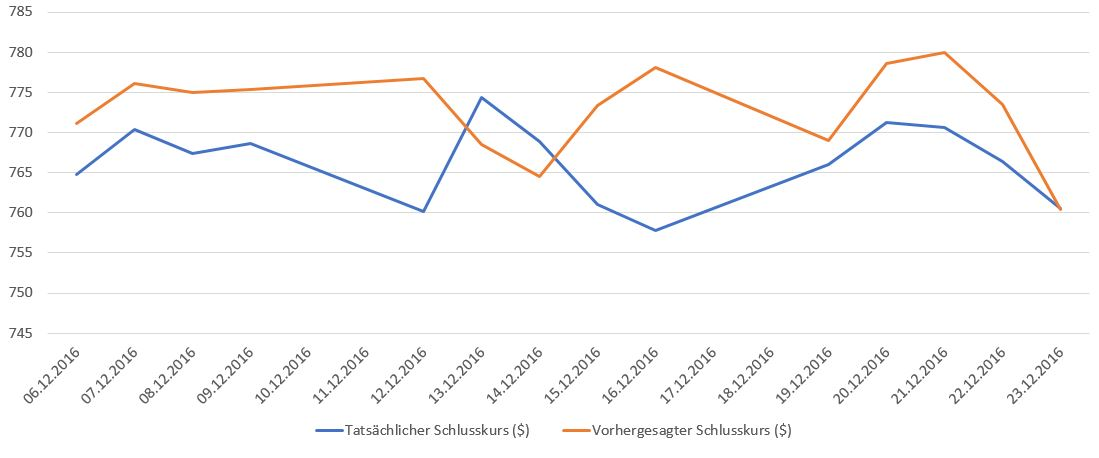
\includegraphics[scale=0.65]{images/Chart.jpg}
    \caption{Tägliche tatsächliche und vorhergesagte Schlusskurse von Amazon}
    \label{fig:chart}
\end{figure}

Eine weitere Methode, um die Qualität der Vorhersagen zu beurteilen ist die Berechnung des Errors der mittleren quadratischen Abweichung (engl. mean squared error). Dafür werden die Abweichungen zwischen den tatsächlichen und den vorhergesagten Schlusskursen quadriert und zum Schluss durch die Anzahl der Vorhersagen geteilt. Für den Error ergibt sich folgender Wert:

\begin{align*}
    MSE &= \frac{1264.74}{14} \\
    MSE &= 90.34
\end{align*}

Somit ergibt sich eine durchschnittliche Abweichung von 90.34, was für einen durchschnittlichen Kurs von etwa 766.28\$ sehr hoch ist. Jedoch sollte auch beachtet werden, dass höhere Abweichungen, wie zum Beispiel am 16.12.2016, auch zu einem höheren durchschnittlichen Fehler führen.

Ferner kann ebenfalls festgestellt werden, dass sich der vorhergesagte Kurs entgegengesetzt zum tatsächlichen Kurs bewegt. So steigt der Kurs des ML-Modells beispielsweise im Zeitraum vom 14. bis 16.12.2016, während in diesem Zeitraum der tatsächliche Kurs fällt. 


Da die Trainingsdaten aus den Jahren 2010 bis 2016 stammen, ist es nicht möglich, mit diesem Modell den morgigen Kurs einer Aktie vorherzusagen. Dazu müssten Trainingsdaten verwendet werden, die nur wenige Monate in der Vergangenheit liegen. Da der Datensatz, der in diesem Projekt verwendet wurde, jedoch nur Informationen bis Ende 2016 beinhaltet, können damit auch nur Vorhersagen in diesem Zeitraum getroffen werden.

Abschließend lässt sich zusammenfassen, dass Aktienkurse durchaus von einem ML-Modell vorhergesagt werden können. Jedoch sollten dabei weitaus mehr Faktoren in das Trainieren des Modells einfließen. Zu solchen Faktoren gehören beispielsweise Prognosen von Banken oder Vermögensverwaltern, Prognosen, die sich positiv oder negativ auf den Aktienkurs auswirken oder ob sich das Unternehmen mitten in einer Krise, wie zum Beispiel der Coronapandemie, befindet. Somit lässt sich sagen, dass der Verlauf einer Aktie nicht nur von mathematischen und statistischen Faktoren abhängt, sondern auch durch psychologische oder extern Rahmenbedingungen beeinflusst werden kann.
		\chapter{Fazit und Ausblick}\label{chp:fazit-und-ausblick}
Für das Vorhersagen von dem Schlusskurs einer Aktie wurde in dieser Ausarbeitung ein ML-Modell in Form einer linearen Regression entwickelt, welches mehrere unabhängige Variablen entgegennimmt. Zu diesen Variablen gehören unter anderem der Eröffnungs-, der Schlusskurs oder der höchste Kurs einer Aktie an einem bestimmten Handelstag. Um den Schlusskurs für darauffolgende Tage vorherzusagen, wurde das Modell mit den Variablen trainiert. Im Anschluss werden Vorhersagen für die Schlusskurse getroffen.

Die Evaluierung zeigte auf, dass sich die Vorhersagen der Schlusskurse weitestgehend in dem Bereich der tatsächlichen Schlusskurse befinden. Neben gelegentlichen Ausreißern traten ebenfalls Vorhersagen auf, die nahezu identisch mit dem tatsächlichen Schlusskurs waren. Dennoch wird abschließend festgehalten, dass ein solches Modell nicht verwendet werden sollte, um eine Kaufentscheidung einer Aktie auszusprechen. Da sich der Kurs, der durch das Modell vorhergesagt wird, teilweise gegensätzlich zum tatsächlichen Kurs verhält, kann diese zu hohen Verlusten am Aktienmarkt führen, wenn auf ein solches Modell vertraut wird.

Um die Qualität der Vorhersagen zu verbessern, kann die Anwendung eines anderen Algorithmus in Betracht gezogen werden. Beispielsweise kann mit einem neuronalen Netz gearbeitet werden, mit dem Verbindungen und Abhängigkeiten innerhalb der Trainingsdaten erkannt werden können. 
Eine weitere Verbesserungsmöglichkeit sollte die Berücksichtigung zusätzlicher Faktoren sein, die in das Trainieren des Modells aufgenommen werden, wie zum Beispiel die aktuelle Marktsituation oder Wirtschaftsnachrichten. Jedoch sollte stets festgehalten werden, dass sich der Aktienmarkt sehr schwer gezielt beeinflussen und vorhersagen lässt.

		% \include{content/06_chapter/test/01_Einleitung.tex}
		% \chapter{CRISP-DM}\label{chp:crisp}

Für den Verlauf dieser Arbeit wird eine Vorgehensweise aus dem Bereich des Data Mining verwendet, da diese gute Anwendungsmöglichkeiten für Projekte im Bereich ML bietet. Diese wird \ac{CRISP-DM} genannt. Der CRISP-DM wird verwendet, um den Lebenszyklus von Daten innerhalb eines Data Mining Projekts zu modellieren und ein dafür geeignetes Data Mining-Modell zu entwickeln. Der Prozess wird dabei in sechs verschiedene Phasen unterteilt, die unterschiedliche Ziele verfolgen \parencite[vgl.][S. 1]{.Wirth}.

\begin{figure}[H]
	\centering
	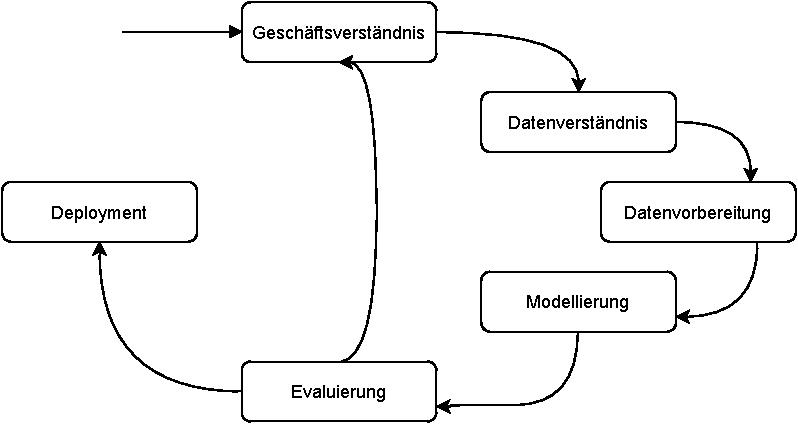
\includegraphics[scale=0.9]{images/CRISP.pdf}
	\caption{Ablauf eines CRISP-DM: Eigene Abbildung in Anlehnung an \parencite[][S. 5]{.Wirth}}
	\label{figure:ablauf-crisp-dm}
\end{figure}

In der ersten Phase geht es darum, die Ziele und die Anforderungen des Projekts zu untersuchen und diese in ein Data Mining-Problem zu übertragen. Anschließend muss sich der Entwickler mit den Daten vertraut machen. Dazu gehört beispielsweise das Gewährleisten der Datenqualität oder Erkenntnisse über die Daten, wie zum Beispiel deren Ursprung, zu sammeln. Nachdem die Daten untersucht wurden, werden diese so vorbereitet, dass sie in das ML-Modell eingefügt und mit ihnen gearbeitet werden kann. Dazu gehört unter anderem, doppelt vorkommende Datensätze oder Ausreißer zu entfernen. Anschließend kann damit begonnen werden, das Modell zu erstellen und die Ergebnisse zu evaluieren. Stellt sich nach der Evaluation heraus, dass nicht alle Anforderungen an das Modell erfüllt wurden, wird erneut damit begonnen, die Anforderungen zu definieren und die Daten zu analysieren, vorzubereiten und ein neues Modell zu erstellen. Erst nachdem alle Anforderungen erfüllt wurden, kann das Modell für den produktiven Gebrauch verwendet werden \parencite[vgl.][S. 5ff.]{.Wirth}.

% An diesen Phasen wird sich der Aufbau dieser Arbeit orientieren. In \vref{chp:problemanalyse-und-datenvorbereitung} wird damit begonnen, das vorliegende Problem zu analysieren und die Daten vorzubereiten. Anschließend werden in \vref{chp:entwicklung-verschiedener-loesungsansaetze} mögliche Modelle und Lösungsansätze entwickelt und in \vref{chp:evaluierung-2} analysiert und evaluiert. Da der Fokus dieser Arbeit auf der Erörterung der Sinnhaftigkeit von Anwendungen von Filtertechniken liegt, wird die Phase des Deployments nicht beachtet und ausgelassen. Auch eine erneute Analyse des Datenverständnisses wird in dieser Arbeit nicht thematisiert. Die Modellierung entspricht dabei der Entwicklung verschiedener Filtertechniken.
		% \chapter{Geschäftsverständnis}\label{chp:geschaeftsverstaendnis}
Die Vorhersage von Aktienkursen ist ein wichtiges Finanzthema, das seit vielen Jahren die Aufmerksamkeit der Forscher auf sich zieht. Dabei wird davon ausgegangen, dass die in der Vergangenheit öffentlich zugänglichen grundlegenden Informationen einen gewissen prädiktiven Einfluss auf die zukünftigen Aktienrenditen haben \parencite[vgl.][S. 1]{.2013}.

Um die Aktienkurse vorherzusagen, existieren grundsätzlich zwei Methoden: die fundamentale und die technische Analyse \parencite[vgl.][S. 26f]{Petrusheva.2016}. Im Bereich der Fundamentalanalyse werden Handelsregeln auf Grundlage der Informationen über Makroökonomie und der Industrie des Unternehmens hergeleitet \parencite[vgl.][S. 1]{.2013}. Diese Art von Analyse geht davon aus, dass der Preis einer Aktie von ihrem inneren Wert und der erwarteten Kapitalrendite abhängt \parencite[vgl.][S. 453]{Tsang.2007}. Somit kann bei dieser Methode beispielsweise anhand der finanziellen Lage, der Liquidität oder der Attraktivität der Branche bewerten, ob eine Aktie Potenzial hat, in der kommenden Zeit zu steigen.

Bei der technischen Analyse hingegen werden Handelsregeln auf Grundlage historischer Daten von Aktienkursen und -volumen entwickelt \parencite[vgl.][S. 1]{.2013}. Diese Methode der Analyse bezieht sich auf verschiedene Methoden, die darauf abzielen, künftige Kursbewegungen anhand von vergangener Aktienkurse und -volumen vorherzusagen. Sie beruht auf der Annahme, dass sich in der Vergangenheit liegende Muster von Aktienkursen wiederholen und dass zukünftige Marktrichtungen anhand von der Untersuchung historischer Kursdaten ermittelt werden können \parencite[vgl.][S. 454]{Tsang.2007}. Bei dieser Methode werden Verfahren wie Trendanalysen, Chartmuster oder technische Indikatoren wie der \ac{MACD} oder Oszillatoren verwendet \parencite[vgl.][S. 293ff]{Mondello.2017}.

Mithilfe dieser Methoden werden Aktienkurse vorausgesagt, um beispielsweise den perfekten Zeitpunkt zu finden, um in die Investition eines Unternehmen einzusteigen oder eine Aktie zu verkaufen, um den Verlust von sinkenden Aktienkursen vorzubeugen. Da diese methodischen Analysen keine Garantie für den Verlauf einer Aktie garantieren, ergibt sich die Überlegung, Aktienkurse mithilfe eines ML-Modells vorherzusagen.
		% \chapter{Datenverständnis}\label{chp:datenverstaendnis}
Bei dem verwendeten Datensatz handelt es sich um eine Sammlung von Unternehmen der \ac{NYSE}, von denen mehrere Kennzahlen des Aktienkurses und des Handelsvolumen gesammelt wurden. Innerhalb dieses Datensatzes wurden Informationen im Zeitraum vom 4. Januar 2010 bis zum 30. Dezember 2016 gesammelt. Dabei wurden nur die Wochentage Montag bis Freitag berücksichtigt, welche keine Feiertage waren. Folglich werden nur reguläre Handelstage an der Börse mit in die Berechnungen aufgenommen. Insgesamt wurden Daten von 501 Unternehmen gesammelt. Bei diesen Daten handelt es sich um folgende Variablen:

\begin{itemize}
    \item Das \textbf{Datum} verweist auf den Tag, an dem die Daten für ein bestimmtes Unternehmen gemessen wurden.
    \item In dem Feld \textbf{Symbol} ist die Abkürzung des Unternehmens gespeichert. Beispielsweise wird für das Unternehmen Amazon die Abkürzung ``AMZN'' hinterlegt.
    \item Der \textbf{Eröffnungskurs} gibt an, mit welchem Kurs die Aktien in den Handelstag gestartet ist.
    \item In der Variable \textbf{Schlusskurs} wird gespeichert, mit welchem Kurs die Aktie den Handelstag beendet hat.
    \item Das \textbf{Hoch} und \textbf{Tief} einer Aktien beschreiben den höchsten, beziehungsweise niedrigsten Kurs, den die Aktien an dem entsprechenden Tag verzeichnet hat.
    \item Das \textbf{Volumen} verweist auf die Anzahl der Aktien eines Unternehmens, die an dem Handelstag gehandelt wurden.
\end{itemize}

Da sich der Zeitraum der gesammelten Daten nur auf 2010 bis 2016 erstreckt, können mit diesem Modell nur Aktienkurse vorhergesagt werden, welche sich auch in diesem Zeitintervall befinden. Um den aktuellen Aktienkurs einer Aktie durch das Modell vorherzusagen, müssten auch aktuelle Daten gesammelt werden. Jedoch werden in \cref{chp:evaluierung} die tatsächlichen Schlusskurse im selbigen Zeitraum mit den von dem Modell vorhergesagten Schlusskursen verglichen.
		% \include{content/06_chapter/Datenvorbreitung.tex}
		% \chapter{Modellierung}\label{chp:modellierung}
Für das Trainieren des Modells wird eine lineare Regression verwendet. Diese wird ebenfalls von der Bibliothek scikit-learn zur Verfügung gestellt. Das Ziel einer linearen Regression ist es, eine erklärende, abhängige Variable Y durch eine oder mehrere unabhängige Variablen X zu erklären und zu zeigen, wie sich Y bei der Veränderung von X ändert \parencite[vgl.][S. 2]{.2010}. Eine lineare Regression lässt sich durch folgende Formel ausdrücken \parencite[vgl.][S. 1]{Montgomery.2021}:

\begin{equation*}
    y = \beta_0 + \beta_n \cdot x_n
\end{equation*}

Dabei handelt es sich bei $y$ um die abhängige Variable und bei $x_n$ um die beschreibenden, beziehungsweise die unabhängigen Variablen.

Übertragen auf das Problemfeld der Vorhersage von Aktienkursen entspricht der Schlusskurs einer Aktie an einem Tag also der abhängigen Variable. Diese hängt über eine Funktion von den Eingangsgrößen, also den unabhängigen oder auch erklärenden Variablen, ab. Zu den erklärenden Variablen gehören der Schluss- und Eröffnungskurs, das Tageshoch und -tief sowie das Handelsvolumen einer Aktie für einen Handelstag.


Mit der Methode \textit{fit}\footnote{https://scikit-learn.org/stable/modules/generated/sklearn.linear\_model.LinearRegression.html} werden dem Modell die x- und y-Werte der Trainingsdaten übergeben. Die x-Daten entsprechen dabei den standardisierten Variablen, mit denen der Aktienkurs vorhergesagt werden soll. Diese sind unter anderem der Eröffnungskurs, das Handelsvolumen oder das Tageshoch. In den y-Werten ist jeweils hinterlegt, mit welchem Kurs die jeweilige Aktie an diesem Tag geschlossen hat. Mit diesen Informationen wird das Modell nun trainiert, damit es für nicht bekannte Eingangsvariablen einen Aktienkurs vorhersagen kann.

Nun können mit der Methode \textit{predict} die Schlusskurse der zu Beginn ausgesuchten Aktie vorhergesagt werden. Dafür wird der Methode der kleine Datensatz übergeben, der die 18 Zeilen enthält, dessen Schlusskurse vorhergesagt werden sollen. Als Ergebnis wird eine Liste zurückgegeben, welche die vorhergesagten Schlusskurse enthält. 
		% \chapter{Evaluierung}\label{chp:evaluierung}
Um die Qualität der Vorhersagen zu bewerten, werden nun die tatsächlichen Schlusskurse mit den vorhergesagten Schlusskursen der Aktien von Amazon verglichen. Die vorhergesagten Schlusskurse beziehen sich auf den Zeitraum vom 6. Dezember bis zum 23. Dezember 2016.

\begin{table}
    \begin{center}
        \begin{tabular}{||c c c c||} 
            \hline
            Datum & \parbox[c]{3.5cm}{\textbf{Tatsächlicher Schlusskurs in \$}} & \parbox[c]{3.5cm}{\textbf{Vorhergesagter Schlusskurs in \$}} & \parbox[c]{3.5cm}{\textbf{Quadratische Abweichung}}\\ [0.5ex] 
        \hline\hline
        06.12.2016 & 764.72 & 771.09 & 40.58 \\ 
    \hline
    07.12.2016 & 770.42 & 776.11 & 32.38 \\
    \hline
    08.12.2016 & 767.33 & 774.92 & 57.61 \\
    \hline
    09.12.2016 & 768.66 & 775.35 & 44.76 \\
    \hline
    12.12.2016 & 760.12 & 776.68 & 274.23 \\ 
    \hline
    13.12.2016 & 774.34 & 768.52 & 33.87 \\
    \hline
    14.12.2016 & 768.82 & 764.50 & 18.66 \\
    \hline
    15.12.2016 & 761.00 & 773.14 & 147.38 \\
    \hline
    16.12.2016 & 757.77 & 778.07 & 412.09 \\
    \hline
    19.12.2016 & 766.00 & 769.03 & 9.18 \\
    \hline
    20.12.2016 & 771.22 & 778.54 & 53.58 \\
    \hline
    21.12.2016 & 770.60 & 780.01 & 88.55 \\
    \hline
    22.12.2016 & 766.34 & 773.54 & 51.84 \\
    \hline
    23.12.2016 & 760.59 & 760.42 & 0.03 \\[1ex]
\end{tabular}
\caption{Vergleich tatsächlicher und vorhergesagter Schlusskurse der Aktie von Amazon}
\label{tab:evaluierung}
\end{center}
\end{table}


Für die tatsächlichen und durch das ML-Modell vorhergesagten Schlusskurse von Amazon in diesem Zeitraum ergeben sich die in \cref{tab:evaluierung} abgebildeten Werte.
Diese zeigt auf, dass sich die durch das ML-Modell vorhergesagten Aktienkurse teilweise im Bereich der tatsächlichen Schlusskurse befindet, die Abweichungen von der Realität einiger Vorhersagen jedoch sehr hoch sind. Außerdem werden in diesem Modell nicht Einflüsse beachtet, die den Verlauf einer Aktie stark beeinflussen könnten. Zu solchen Einflüssen zählen beispielsweise das Erhalten eines umfangreichen Kundenauftrags, Prognosen, die einen Gewinnrückgang erwarten oder steigende Zinsen an den Kapitalmärkten. \cref{fig:chart} zeigt die grafische Darstellung der Schlusskurse im Zeitraum vom 06.12.2016 bis zum 23.12.2016.

\begin{figure}[H]
    \centering
    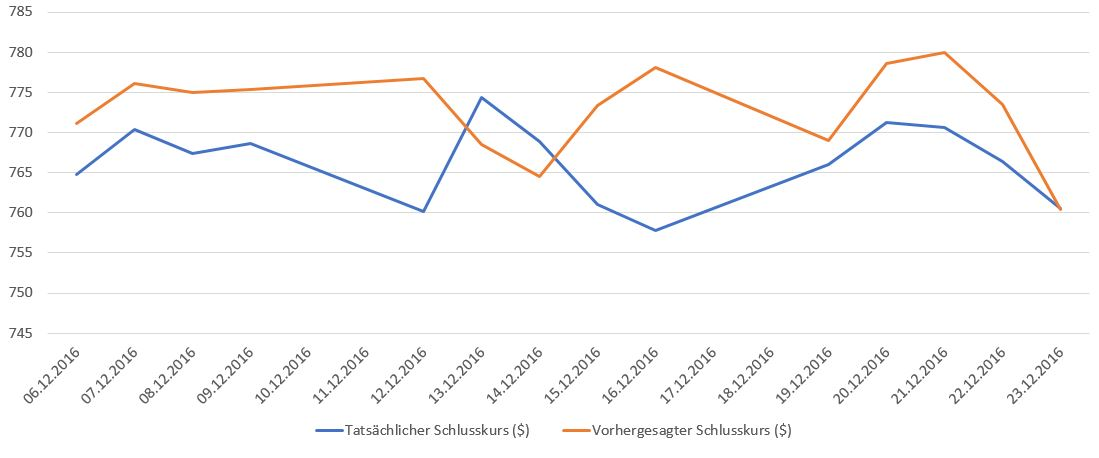
\includegraphics[scale=0.65]{images/Chart.jpg}
    \caption{Tägliche tatsächliche und vorhergesagte Schlusskurse von Amazon}
    \label{fig:chart}
\end{figure}

Eine weitere Methode, um die Qualität der Vorhersagen zu beurteilen ist die Berechnung des Errors der mittleren quadratischen Abweichung (engl. mean squared error). Dafür werden die Abweichungen zwischen den tatsächlichen und den vorhergesagten Schlusskursen quadriert und zum Schluss durch die Anzahl der Vorhersagen geteilt. Für den Error ergibt sich folgender Wert:

\begin{align*}
    MSE &= \frac{1264.74}{14} \\
    MSE &= 90.34
\end{align*}

Somit ergibt sich eine durchschnittliche Abweichung von 90.34, was für einen durchschnittlichen Kurs von etwa 766.28\$ sehr hoch ist. Jedoch sollte auch beachtet werden, dass höhere Abweichungen, wie zum Beispiel am 16.12.2016, auch zu einem höheren durchschnittlichen Fehler führen.

Ferner kann ebenfalls festgestellt werden, dass sich der vorhergesagte Kurs entgegengesetzt zum tatsächlichen Kurs bewegt. So steigt der Kurs des ML-Modells beispielsweise im Zeitraum vom 14. bis 16.12.2016, während in diesem Zeitraum der tatsächliche Kurs fällt. 


Da die Trainingsdaten aus den Jahren 2010 bis 2016 stammen, ist es nicht möglich, mit diesem Modell den morgigen Kurs einer Aktie vorherzusagen. Dazu müssten Trainingsdaten verwendet werden, die nur wenige Monate in der Vergangenheit liegen. Da der Datensatz, der in diesem Projekt verwendet wurde, jedoch nur Informationen bis Ende 2016 beinhaltet, können damit auch nur Vorhersagen in diesem Zeitraum getroffen werden.

Abschließend lässt sich zusammenfassen, dass Aktienkurse durchaus von einem ML-Modell vorhergesagt werden können. Jedoch sollten dabei weitaus mehr Faktoren in das Trainieren des Modells einfließen. Zu solchen Faktoren gehören beispielsweise Prognosen von Banken oder Vermögensverwaltern, Prognosen, die sich positiv oder negativ auf den Aktienkurs auswirken oder ob sich das Unternehmen mitten in einer Krise, wie zum Beispiel der Coronapandemie, befindet. Somit lässt sich sagen, dass der Verlauf einer Aktie nicht nur von mathematischen und statistischen Faktoren abhängt, sondern auch durch psychologische oder extern Rahmenbedingungen beeinflusst werden kann.
	
	
	% -- Einbinden des Literaturverzeichnisses 
	\cleardoublepage												% Beendet eine Seite
	\renewcommand*{\chapterpagestyle}{plain}						% Kapitel-Style wird auf plain gestellt 
	\pagestyle{plain}												% Seiten-Style wird auf plain gestellt			
	\pagenumbering{Roman}                   						% Römische Seitenzahlen
	\setcounter{page}{\numexpr\value{savepage}+1}					% Zähler der römischen Zahlen wird inkrementiert
	\printbibliography												% Literaturverzeichnis wird erstellt
	
	% -- Einbinden des Glossars
	\printglossary[style=altlist,title=Glossar]						% Glossar wird erstellt

    % -- Einbinden von Anhängen
    \begin{appendices}
		% Current file is content/07_appendix/index.tex

\renewcommand{\indexname}{Stichwortverzeichnis}
\printindex

	\ifthenelse{\boolean{abgabeVersion}}
	{}
	{
		\chapter{Uninteressanter Anhang}
Dies Anhang besitzt eigentlich keinen Sinn, außer einen Platzhalter im Inhaltsverzeichnis zu erzeugen.
	} 	
    \end{appendices}
\end{document}